\documentclass[12pt,a4paper]{article}
\usepackage[utf8]{inputenc}
\usepackage[vietnamese]{babel}
\usepackage{amsmath, amssymb, amsfonts}
\usepackage{graphicx}
\usepackage{float}
\usepackage{hyperref} % Tạo mục lục có thể click
\usepackage{listings} % Để chèn code Python
\usepackage{geometry}
 \geometry{a4paper, margin=2.5cm}
 
\title{BÁO CÁO ĐỒ ÁN MÔN HỌC}
\begin{document}
\maketitle
% --- 1. TRANG BÌA ---
\begin{titlepage}
    \centering
    \vspace*{1cm}
    {\Large \textbf{TRƯỜNG ĐẠI HỌC KHOA HỌC TỰ NHIÊN, ĐHQG-HCM} \par}
    {\Large \textbf{KHOA CÔNG NGHỆ THÔNG TIN} \par}
    \vspace{2cm}
    \includegraphics[width=0.3\textwidth]{logo_hcmus.png}\par 
    \vspace{1.5cm}
    {\huge \textsf{\textbf{ĐỒ ÁN 1: MA TRẬN VÀ TÍNH TOÁN KHOA HỌC}} \par}
    \vspace{2cm}
    \begin{flushright}
        \textbf{Giảng viên hướng dẫn:} Th.S Lê Nhựt Nam \\
        \textbf{Sinh viên thực hiện:} \\
        24120430 - Trần Thanh Sơn \\
        24120389 - Từ Quốc Nghĩa \\
        21120449 - Nguyễn Văn Hậu \\
        24120263 - Đỗ Ngọc Gia Bảo \\
        23120027 - Nguyễn Hải Đăng \\
        \textbf{Nhóm:} 15
    \end{flushright}
    \vfill
    {\large \today}
\end{titlepage}

% --- 2. MỤC LỤC ---
\newpage
\tableofcontents
\newpage

\section{Phần 1 Phép khử Gauss và Các Ứng Dụng}
\subsection{Tổng hợp lý thuyết}
\subsubsection{Các khái niệm cơ bản}
\paragraph{Ma trận tăng cường}
Xét hệ phương trình tuyến tính $$Ax = b \text{ với } A \in \mathbb{R}^{m \times n}, x \in \mathbb{R}^n, b \in \mathbb{R}^m$$

Để giải hệ Ax = b ta lập ma trận tăng cường [A|b]\\
$$[A | b] = 
\left( \begin{array}{cccc|c}
a_{11} & a_{12} & \cdots & a_{1n} & b_1 \\
a_{21} & a_{22} & \cdots & a_{2n} & b_2 \\
\vdots & \vdots & \ddots & \vdots & \vdots \\
a_{m1} & a_{m2} & \cdots & a_{mn} & b_m
\end{array} \right)
$$

\paragraph{Các phép biến đổi sơ cấp trên dòng}
\begin{enumerate}
    \item $R_i \leftrightarrow R_j$: Hoán đổi dòng $i$ và dòng $j$.
    \item $R_i \leftarrow c \cdot R_i, (c \neq 0)$: Nhân dòng $i$ với hằng số $c$.
    \item $R_i \leftarrow R_i + c \cdot R_j$: Cộng $c$ lần dòng $j$ vào dòng $i$.
\end{enumerate}

\paragraph{Dạng bậc thang (REF và RREF)}
\subparagraph{Dạng bậc thang dòng — REF}
\noindent Ma trận $U$ được gọi là có dạng \textbf{bậc thang dòng} (Row Echelon Form) nếu thỏa mãn hai điều kiện sau:
\begin{itemize}
    \item Mọi dòng toàn số 0 (nếu có) đều nằm phía dưới các dòng khác 0.
    \item Phần tử chỉ huy của mỗi dòng khác 0 nằm ở cột bên phải so với phần tử chỉ huy của dòng ngay phía trên nó.
\end{itemize}

\textit{Ví dụ:}
\[
U = \begin{pmatrix}
\mathbf{1} & 2 & 1 & 1 \\
0 & 0 & \mathbf{3} & 5 \\
0 & 0 & 0 & \mathbf{9} \\
0 & 0 & 0 & 0
\end{pmatrix}
\]

\subparagraph{Dạng bậc thang dòng rút gọn — RREF}
\noindent Ma trận $R$ được gọi là có dạng \textbf{bậc thang dòng rút gọn} (Reduced Row Echelon Form - RREF) nếu nó thỏa mãn các điều kiện của dạng bậc thang dòng (REF) và thêm hai điều kiện sau:

\begin{itemize}
    \item Mỗi phần tử chỉ huy (pivot) đều bằng 1.
    \item Trong mỗi cột chứa pivot, tất cả các phần tử khác (ngoài chính pivot đó) đều bằng 0.
\end{itemize}

\textit{Ví dụ:}
\[
R = \begin{pmatrix}
\mathbf{1} & 0 & 2 & 0 \\
0 & \mathbf{1} & 3 & 0 \\
0 & 0 & 0 & \mathbf{1} \\
0 & 0 & 0 & 0
\end{pmatrix}
\]

\subsubsection{Kỹ thuật Partial Pivoting (Chọn phần tử chốt)}
Quy trình tại bước $k$: Tìm dòng $p$ (từ dòng $k$ đến $n$) có $|a_{pk}|$ lớn nhất. Hoán đổi dòng $k$ và dòng $p$. Nếu $|a_{pk}| < \epsilon$ (một số rất bé, ví dụ $10^{-12}$), ta coi như cột đó không có pivot.

\subsection{Các ứng dụng của phép khử Gauss}
\subsubsection{Giải hệ phương trình (Gaussian Elimination)}
\paragraph{\texttt{\textbf{gaussian\_eliminate(A, b)}}}
Sử dụng thuật toán Gauss-Jordan kết hợp với kỹ thuật chọn phần tử chốt (Partial Pivoting) để biến đổi ma trận tăng cường $[A | b]$ về dạng bậc thang dòng rút gọn (RREF). Quá trình thực hiện bao gồm các bước chính sau:
\begin{itemize}
\item \textbf{Khởi tạo:} Ghép ma trận hệ số $A$ và vector (hoặc ma trận) $b$ thành ma trận tăng cường $M$.

\item \textbf{Chọn phần tử chốt (Partial Pivoting):} Tại mỗi cột $k$, tìm dòng có giá trị tuyệt đối lớn nhất từ dòng $k$ trở xuống để làm phần tử chốt ($pivot$). Điều này giúp giảm thiểu sai số làm tròn và tránh trường hợp chia cho $0$.

\item \textbf{Biến đổi sơ cấp:}

    \begin{itemize}
    \item Hoán đổi dòng hiện tại với dòng chứa phần tử chốt (nếu cần).
    \item Chuẩn hóa dòng chốt bằng cách chia toàn bộ các phần tử trong dòng cho $pivot$ để đưa giá trị tại vị trí $(k, k)$ về bằng $1$.
    \item Khử tất cả các phần tử khác trong cột $k$ (cả phía trên và phía dưới dòng chốt) về bằng $0$.
    \end{itemize}
    
\item \textbf{Xử lý nghiệm:} Sau khi đưa về dạng RREF, thuật toán sẽ kiểm tra tính nhất quán của hệ phương trình để trả về kết quả là nghiệm duy nhất, thông báo vô nghiệm hoặc vô số nghiệm.\end{itemize}

Hàm sẽ trả về một bộ tuple gồm:
\begin{itemize}
\item \textbf{RREF\_matrix} Ma trận RREF
\item \textbf{x} Nghiệm hệ phương trình (list) hoặc chuỗi báo lỗi ("Vo nghiem"...).
\item \textbf{swap\_count} Số lần hoán đổi dòng.
\item \textbf{det\_multiplier:}  Tích các pivot (dùng để tính định thức).
\end{itemize}

\paragraph{\texttt{\textbf{back\_substitution(U,c)}}}
Thuật toán thực hiện giải hệ phương trình tam giác trên $Ux = c$ bằng cách tính ngược từ ẩn số cuối cùng và thế dần các giá trị đã biết lên các dòng phía trên:
\begin{equation}
x_i = \frac{1}{M_{ii}} \left( M_{i, m+1} - \sum_{j=i+1}^{n} M_{ij} x_j \right), \quad i = n, n-1, \dots, 1
\end{equation}

Thuật toán được cài đặt trong hàm \texttt{back\_substitution} theo các bước logic sau:
\begin{itemize}
    \item \textbf{Khởi tạo mảng nghiệm:} Một danh sách \texttt{solution} có kích thước $m$ được khởi tạo với các giá trị $0.0$ để lưu trữ kết quả của các ẩn số $x_i$.
    
    \item \textbf{Vòng lặp ngược (Backward Loop):} Sử dụng vòng lặp duyệt chỉ số $i$ từ $m-1$ ngược về $0$. Điều này tương ứng với việc giải phương trình từ dưới lên trên.
    
    \item \textbf{Kiểm tra điều kiện khả nghịch:} Tại mỗi bước, thuật toán kiểm tra phần tử chốt $U_{ii}$. Nếu $|U_{ii}| < \epsilon$ (\texttt{EPSILON}), hệ phương trình không có nghiệm duy nhất và một ngoại lệ \texttt{ValueError} sẽ được ném ra để đảm bảo tính an toàn cho chương trình.
    
    \item \textbf{Tính toán giá trị ẩn số:}
    Với mỗi dòng $i$, giá trị nghiệm $x_i$ được tính theo công thức tương tự như lý thuyết:
    $$x_i = \frac{c_i - \sum_{j=i+1}^{m} U_{ij}x_j}{U_{ii}}$$
    Trong đó, tổng $\sum$ (biến \texttt{total} trong code) đại diện cho tích của các hệ số đã biết với các nghiệm đã được tính toán ở các bước trước đó.
\end{itemize}

\subsubsection{Tính định thức}
Sau khi đưa ma trận $A$ về dạng tam giác trên $U$ bằng phép khử Gauss với $s$ lần hoán đổi dòng, định thức được tính theo công thức:
\begin{equation}
    \det(A) = (-1)^s \cdot \prod_{i=1}^{n} u_{ii}
\end{equation}
Trong đó $u_{ii}$ là các phần tử trên đường chéo chính của ma trận sau khi khử.

Từ hàm \texttt{\textbf{gaussian\_eliminate(A, b)}} ta đã có được số lần hoán đổi dòng và tích các pivot. Do đó sau khi \texttt{\textbf{determinant(A)}} gọi \texttt{\textbf{gaussian\_eliminate(A, b)}} sẽ tính được định thức của ma trận là: 
\begin{equation}
    \det(A) = (-1)^{\text{swap\_count}} \cdot \text{det\_multiplier}
\end{equation}

\subsubsection{Tìm ma trận nghịch đảo (Inverse)}
Ma trận $A \in \mathbb{R}^{n \times n}$ khả nghịch khi và chỉ khi $\det(A) \neq 0$. Nghịch đảo $A^{-1}$ được tìm bằng cách thực hiện các phép biến đổi dòng sơ cấp đồng thời trên ma trận ghép $[A \mid I_n]$ cho đến khi đạt được dạng $[I_n \mid A^{-1}]$:

Thuật toán tìm ma trận nghịch đảo trong \texttt{\textbf{inverse(A)}}:
\begin{itemize}
    \item \textbf{Kiểm tra điều kiện:} Đầu tiên, hàm kiểm tra tính vuông của ma trận. Nếu $m \neq n$, hàm trả về thông báo lỗi vì chỉ ma trận vuông mới có khả năng khả nghịch.
    
    \item \textbf{Khởi tạo ma trận ghép:} Sử dụng \textit{list comprehension} để tạo ma trận đơn vị $I_n$. Sau đó, gọi hàm 
    
    \texttt{\textbf{gaussian\_eliminate(A, I)}} để thực hiện biến đổi dòng trên ma trận ghép $[A \mid I_n]$.
    
    \item \textbf{Kiểm tra tính khả nghịch:} Dựa vào giá trị \texttt{det\_multiplier} trả về. Nếu $|\det(A)| < 10^{-9}$, ma trận được coi là suy biến và không có ma trận nghịch đảo.
    
    \item \textbf{Trích xuất kết quả:} Sau khi ma trận ghép đạt dạng $[I_n \mid A^{-1}]$, hàm thực hiện tách lấy các cột từ chỉ số $n$ trở đi ở mỗi dòng để thu được ma trận nghịch đảo:
    
    \begin{lstlisting}[language=Python]
    inv_matrix = [row[n:] for row in RREF_matrix]
    \end{lstlisting}
\end{itemize}

\subsubsection{Tính hạng và cơ sở}
\paragraph{Hạng của ma trận}
Hạng (rank) của ma trận A, ký hiệu rank(A), bằng số dòng
khác 0 trong dạng REF của A, hoặc tương đương, bằng số cột pivot.

\paragraph{Cơ sở của các không gian con}
\begin{itemize}
    \item \textbf{Không gian cột (column space) $\mathcal{C}(A)$:} sinh bởi các cột pivot của $A$ gốc.
    \item \textbf{Không gian dòng (row space) $\mathcal{R}(A)$:} sinh bởi các dòng khác $0$ trong RREF.
    \item \textbf{Không gian nghiệm (null space) $\mathcal{N}(A)$:} tập nghiệm của $Ax = 0$.
\end{itemize}

Thuật toán cài đặt trong \texttt{\textbf{rank\_and\_basis(A)}}:
\begin{itemize}
    \item Thông qua thuật toán Gauss-Jordan, ma trận $A$ được biến đổi về dạng RREF.
    
    \item Dựa trên ma trận RREF, hàm duyệt qua các cột để xác định các cột chứa phần tử chốt (pivot). Danh sách pivot\_cols lưu trữ chỉ số của các cột này.
    
    \item Hạng của ma trận được xác định bằng tổng số lượng cột pivot tìm thấy.

    \item \textbf{Cơ sở không gian cột:} Trích xuất các cột tại vị trí \texttt{pivot\_cols} từ ma trận $A$ ban đầu.

    \item \textbf{Cơ sở không gian dòng:} Lấy các dòng khác không từ ma trận RREF (kiểm tra phần tử khác $0$ dựa trên ngưỡng \texttt{epsilon}).

    \item \textbf{Cơ sở không gian nghiệm:} Giải hệ $Ax=0$ bằng cách gán lần lượt từng biến tự do (cột không chứa pivot) bằng $1$ và tính giá trị các biến cơ sở từ các hệ số tương ứng trong RREF.
\end{itemize}

\subsection{Báo cáo kết quả}
\subsubsection{Cài đặt hàm \texttt{\textbf{verify\_solve(A, b, x\_nhom)}}}
\begin{figure}[H]
    \centering
    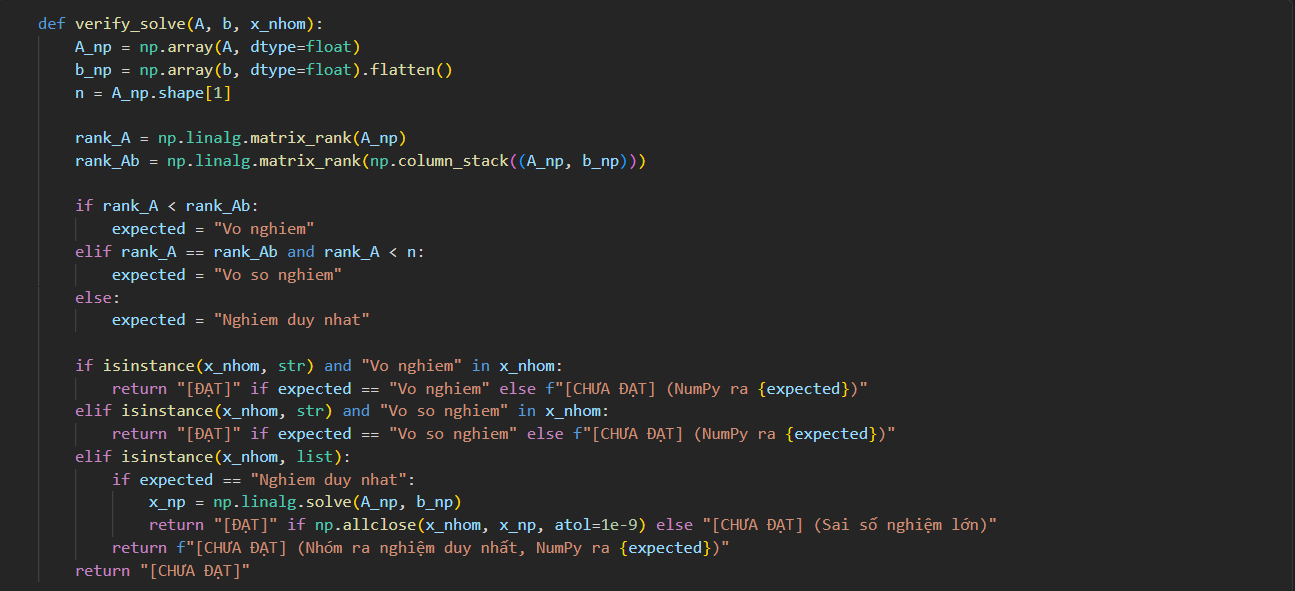
\includegraphics[width=1\linewidth]{image.png}
    \label{fig:placeholder}
\end{figure}

\subsubsection{Các test case}
\begin{figure}[H]
    \centering
    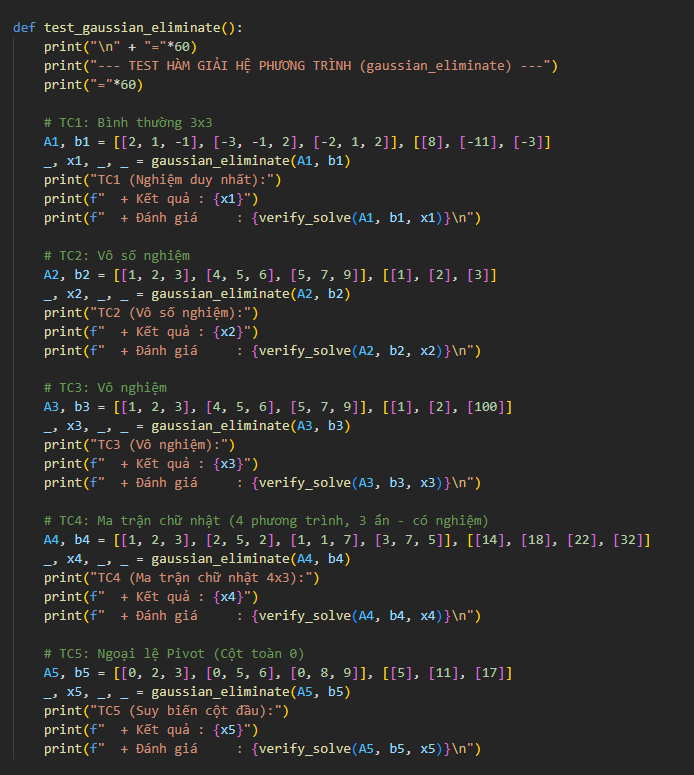
\includegraphics[width=1\linewidth]{image1.png}
    \label{fig:placeholder}
\end{figure}
\subsubsection{Kết quả}
\begin{figure}[H]
    \centering
    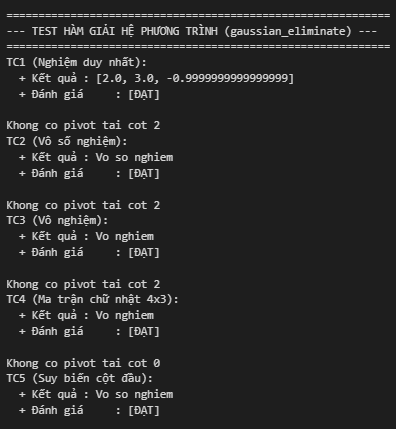
\includegraphics[width=1\linewidth]{image7.png}
    \label{fig:placeholder}
\end{figure}

\subsubsection{Kiểm thử tính định thức}

\paragraph{Cài đặt hàm kiểm thử và các test case} \leavevmode \\

\begin{figure}[H]
    \centering
    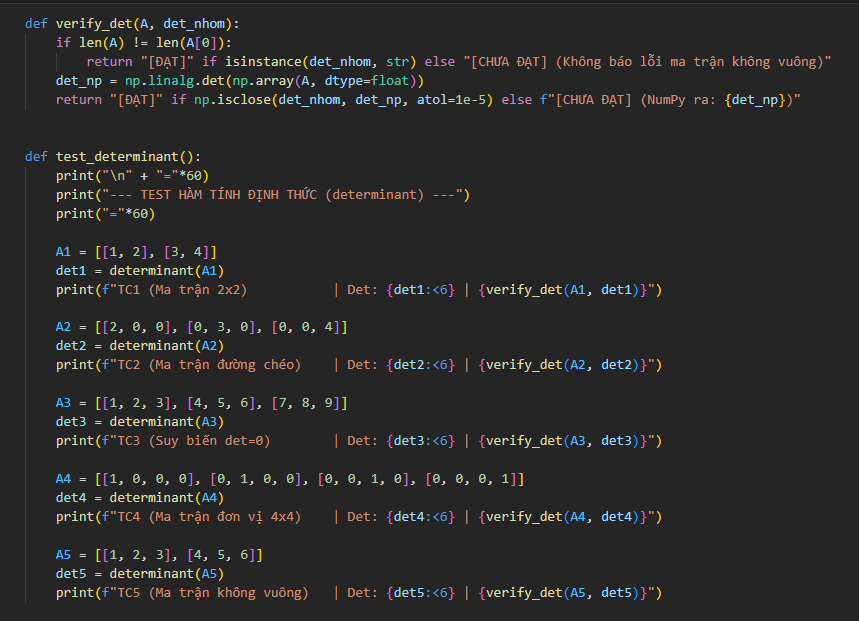
\includegraphics[width=1\linewidth]{image3.png}
    \label{fig:placeholder}
\end{figure}
\paragraph{Kết quả} \leavevmode \\

\begin{figure}[H]
    \centering
    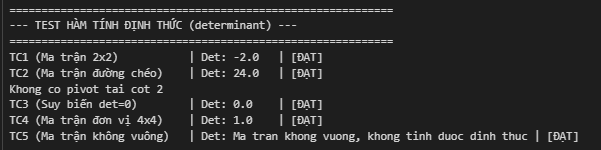
\includegraphics[width=1\linewidth]{image8.png}
    \label{fig:placeholder}
\end{figure}

\subsubsection{Kiểm thử tìm ma trận nghịch đảo}

\paragraph{Cài đặt hàm kiểm thử và các test case} \leavevmode \\

\begin{figure}[H]
    \centering
    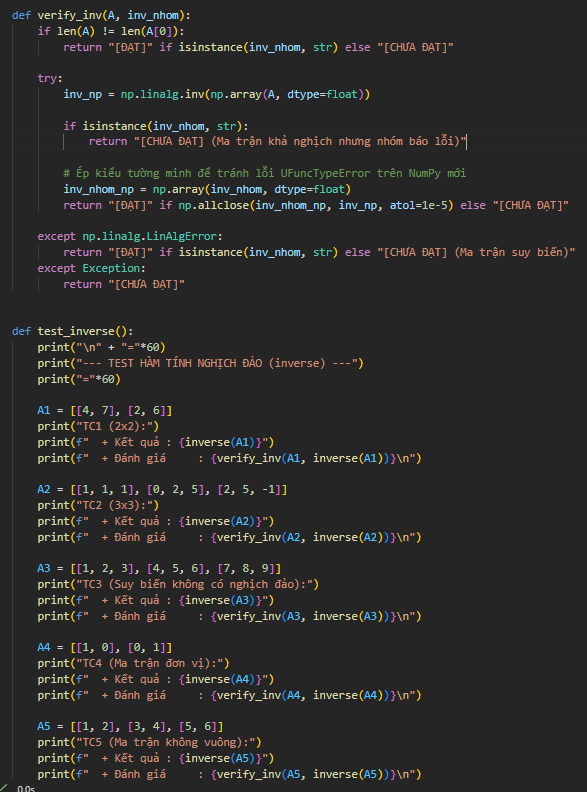
\includegraphics[width=1\linewidth]{image4.png}
    \label{fig:placeholder}
\end{figure}
\paragraph{Kết quả} \leavevmode \\

\begin{figure}[H]
    \centering
    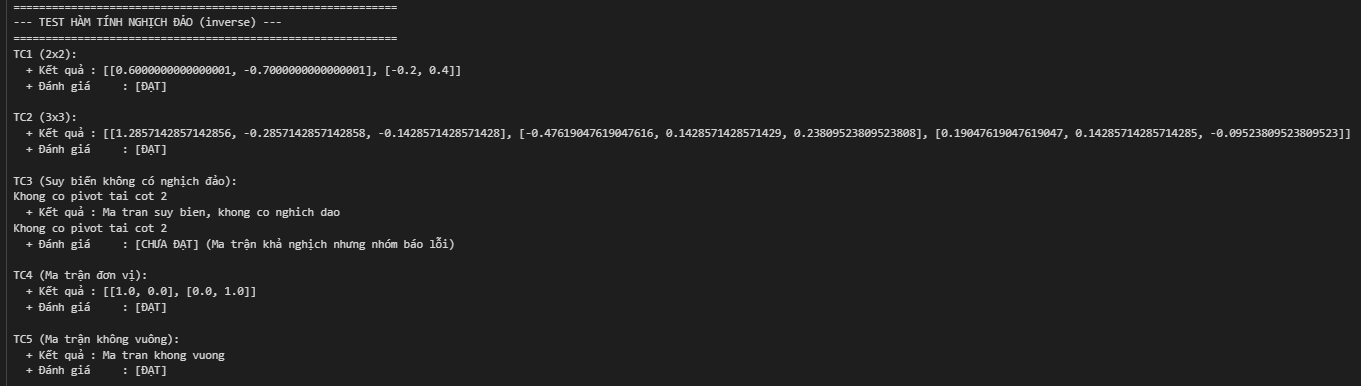
\includegraphics[width=1\linewidth]{image9.png}
    \label{fig:placeholder}
\end{figure}

\subsubsection{Kiểm thử tìm hạng và cơ sở}

\paragraph{Cài đặt hàm kiểm thử và các test case} \leavevmode \\

\begin{figure}[H]
    \centering
    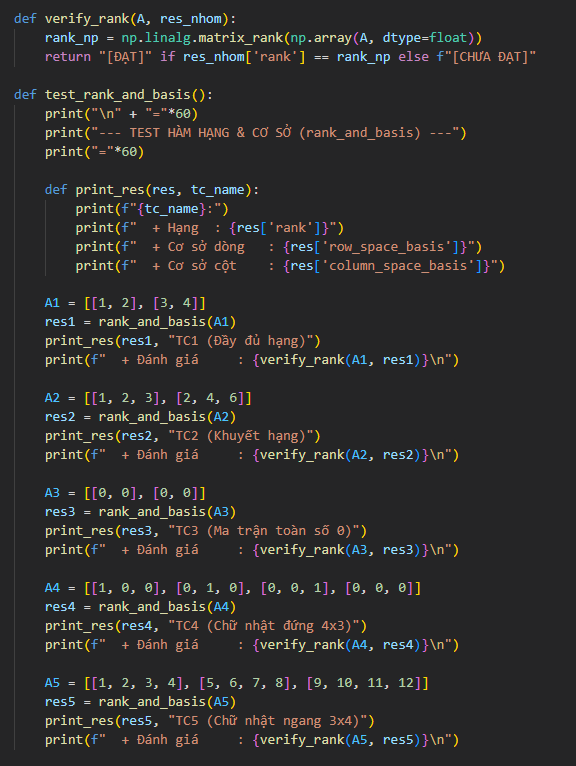
\includegraphics[width=1\linewidth]{image5.png}
    \label{fig:placeholder}
\end{figure}
\paragraph{Kết quả} \leavevmode \\

\begin{figure}[H]
    \centering
    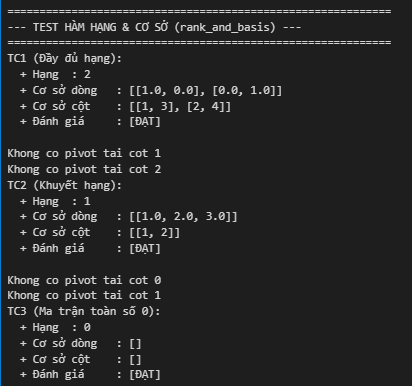
\includegraphics[width=1\linewidth]{image10.png}
    \label{fig:placeholder}
\end{figure}
\begin{figure}[H]
    \centering
    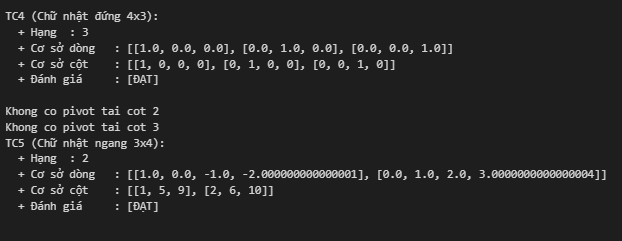
\includegraphics[width=1\linewidth]{image11.png}
    \label{fig:placeholder}
\end{figure}

\subsubsection{Kiểm thử giải hệ tam giác trên}

\paragraph{Cài đặt hàm kiểm thử và các test case} \leavevmode \\

\begin{figure}[H]
    \centering
    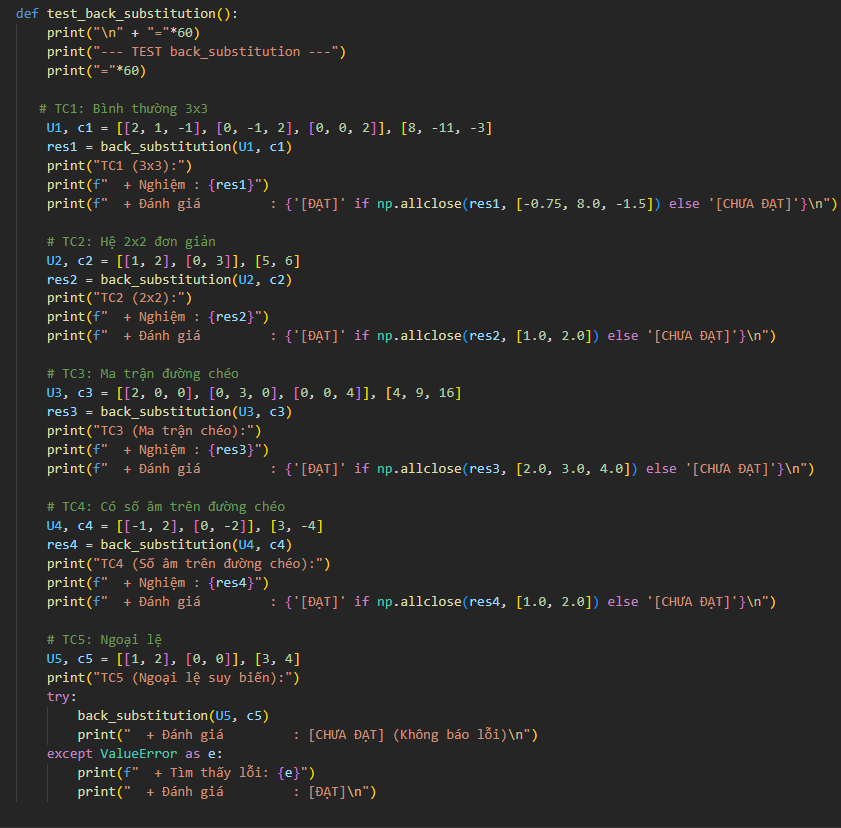
\includegraphics[width=1\linewidth]{image6.png}
    \label{fig:placeholder}
\end{figure}
\paragraph{Kết quả} \leavevmode \\

\begin{figure}[H]
    \centering
    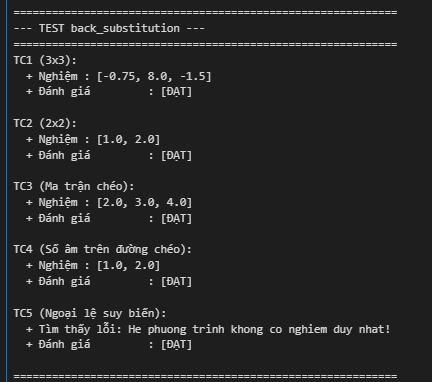
\includegraphics[width=1\linewidth]{image12.png}
    \label{fig:placeholder}
\end{figure}

% --- TÀI LIỆU THAM KHẢO ---
\newpage
\begin{thebibliography}{9}
    \bibitem{strang} Gilbert Strang, \textit{Introduction to Linear Algebra}, 5th Edition, Wellesley-Cambridge Press, 2016.
    \bibitem{anton} Howard Anton, Chris Rorres, \textit{Elementary Linear Algebra}, Wiley, 2013.
    \bibitem{python} Python Software Foundation, \textit{Python Language Reference}, \url{https://www.python.org/}.
    \bibitem{numpy} Harris, C.R. et al., \textit{Array programming with NumPy}, Nature, 2020.
    \bibitem{hcmus} Tài liệu hướng dẫn thực hành Toán ứng dụng, FIT-HCMUS.
\end{thebibliography}

% --- PHỤ LỤC ---
\newpage
\appendix
\section{Mã nguồn chương trình (Bổ sung nếu có)}
% Dùng gói listings để chèn code đẹp hơn
\begin{lstlisting}[language=Python, caption=Hàm Gaussian Eliminate]

\end{lstlisting}
\end{document}


